% !TEX program = xelatex
\documentclass[11pt,a4paper]{article}
\usepackage{fontspec}
\setmainfont{Calibri}
\setmonofont[Scale=0.88]{Consolas}
\newfontfamily\symbolfont{Segoe UI Symbol}
\usepackage{polyglossia}\setdefaultlanguage{polish}
\usepackage[table]{xcolor}
\usepackage{booktabs,longtable,array,geometry,enumitem,graphicx,fancyhdr,caption}
\usepackage[most]{tcolorbox}
\PassOptionsToPackage{hyphens}{url}
\usepackage[hidelinks,unicode]{hyperref}
\emergencystretch=2.5em
\geometry{a4paper,margin=2.1cm,top=2.3cm,bottom=2.3cm}
\setlength{\parindent}{0pt}\setlength{\parskip}{5pt}
\definecolor{apteal}{HTML}{0E7C86}
\definecolor{apteallight}{HTML}{E6F4F5}
\definecolor{apgrey}{HTML}{F3F4F6}
\definecolor{apamber}{HTML}{B45309}
\definecolor{apamberlight}{HTML}{FEF3C7}
\definecolor{apred}{HTML}{B91C1C}
\definecolor{apredlight}{HTML}{FEE2E2}
\definecolor{apgreen}{HTML}{15803D}
\definecolor{apgreenlight}{HTML}{DCFCE7}
\renewcommand{\arraystretch}{1.25}
\captionsetup{font=small,labelfont=bf}
\pagestyle{fancy}\fancyhf{}
\fancyfoot[L]{\small AMPERE POINT — MQTT i OCPP w Q11 z modułem Shelly · opis i test · v1 · 2026-09-25}
\fancyfoot[R]{\small\thepage}
\renewcommand{\headrulewidth}{0pt}
\newtcolorbox{uwaga}[1][Uwaga]{enhanced,breakable,colback=apamberlight,colframe=apamber,title={#1},fonttitle=\bfseries,boxrule=0.6pt,arc=2pt,left=6pt,right=6pt,top=4pt,bottom=4pt}
\newtcolorbox{info}[1][Jak to działa]{enhanced,breakable,colback=apteallight,colframe=apteal,title={#1},fonttitle=\bfseries,boxrule=0.6pt,arc=2pt,left=6pt,right=6pt,top=4pt,bottom=4pt}
\newtcolorbox{wazne}[1][Ważne]{enhanced,breakable,colback=apredlight,colframe=apred,title={#1},fonttitle=\bfseries,boxrule=0.6pt,arc=2pt,left=6pt,right=6pt,top=4pt,bottom=4pt}
\newtcolorbox{przyklad}[1][Przykład liczbowy]{enhanced,breakable,colback=apgreenlight,colframe=apgreen,title={#1},fonttitle=\bfseries,boxrule=0.6pt,arc=2pt,left=6pt,right=6pt,top=4pt,bottom=4pt}
\newtcolorbox{kodbox}{enhanced,breakable,colback=apgrey,colframe=apgrey,boxrule=0pt,arc=2pt,left=5pt,right=5pt,top=3pt,bottom=3pt,fontupper=\ttfamily\footnotesize}
\setlist{nosep,leftmargin=*}
\setcounter{secnumdepth}{2}
\begin{document}

{\LARGE\bfseries MQTT i OCPP w Q11 z modułem Shelly\par}
{\large Jak działają i jak je sprawdziliśmy · AMPERE POINT · 25 września 2026 · oprac. Dawid Cekała\par}
\vspace{4pt}\textcolor{apteal}{\rule{\textwidth}{1.2pt}}

\section*{W skrócie}

\begin{itemize}
\item Moduł Shelly, na razie jako DevKit, siedzi w Q11 w miejscu modułu Tuya WBR3. Rozmawia z mikrokontrolerem ładowarki protokołem Tuya przy 9600 b/s.
\item \textbf{MQTT:} DevKit sam wysyła stan ładowarki do brokera w sieci lokalnej i przez niego przyjmuje polecenia. Limit prądu wysłany przez MQTT Q11 potwierdziła w tej samej sekundzie.
\item \textbf{OCPP 1.6J:} DevKit nie potrafi mówić OCPP sam. Robi to most, czyli program na komputerze, który tłumaczy OCPP na polecenia Shelly. Z serwerem testowym działa rejestracja, stan, pomiary, limit prądu i zdalny start.
\item Oba kanały działają przy wyłączonej chmurze Shelly.
\item Warunek pracy bez internetu to lokalny serwer czasu. Stoi w Dockerze na laptopie.
\item Nie sprawdziliśmy jeszcze pełnej transakcji ładowania w OCPP. Potrzebne jest auto albo symulator pobierający prąd.
\item Test był w sieci biura bez szyfrowania i haseł. W produkcji oba kanały muszą mieć TLS i uwierzytelnianie.
\end{itemize}

\section{Układ całości}

\begin{figure}[h]\centering
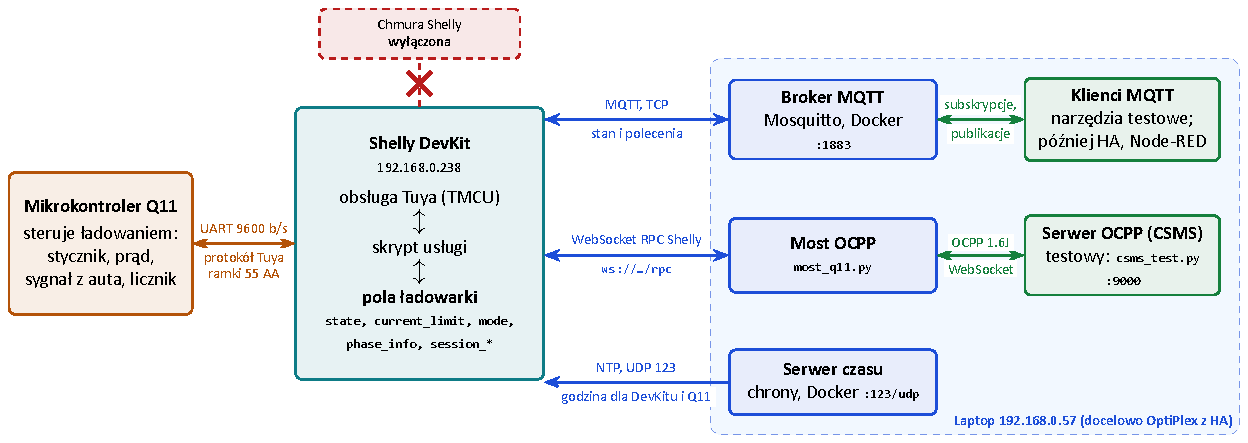
\includegraphics[width=1.00\textwidth]{img/schemat_mqtt_ocpp.pdf}
\caption{Połączenia w teście z 25.09.2026. Chmura Shelly była wyłączona, wszystko działało w sieci biura.}
\end{figure}

\begin{longtable}{>{\raggedright\arraybackslash}p{3.00cm}>{\raggedright\arraybackslash}p{2.87cm}>{\raggedright\arraybackslash}p{2.57cm}>{\raggedright\arraybackslash}p{6.39cm}}
\toprule
\rowcolor{apteallight}\textbf{Element} & \textbf{Gdzie działa} & \textbf{Adres} & \textbf{Rola} \\
\midrule\endhead
\bottomrule\endfoot
Mikrokontroler Q11 & płytka sterująca ładowarki & łącze szeregowe & steruje ładowaniem, mierzy, pilnuje bezpieczeństwa \\
Shelly DevKit & w obudowie Q11, zasilany z płytki & \texttt{192.\allowbreak{}168.\allowbreak{}0.\allowbreak{}238} & tłumaczy protokół Tuya na pola Shelly, wysyła MQTT, przyjmuje polecenia \\
Broker MQTT Mosquitto 2.1.2 & Docker na laptopie & \texttt{192.\allowbreak{}168.\allowbreak{}0.\allowbreak{}57:\allowbreak{}1883} & przekazuje wiadomości między DevKitem a odbiorcami \\
Most OCPP \texttt{most\_q11.py} & Python na laptopie & łączy się do DevKitu i serwera & udaje ładowarkę OCPP i przekłada polecenia na Shelly \\
Serwer OCPP \texttt{csms\_test.py} & Python na laptopie & \texttt{ws:\allowbreak{}/\allowbreak{}/\allowbreak{}localhost:\allowbreak{}9000} & udaje system operatora, zapisuje każdą wiadomość \\
Serwer czasu chrony & Docker na laptopie & \texttt{192.\allowbreak{}168.\allowbreak{}0.\allowbreak{}57:\allowbreak{}123}, UDP & podaje godzinę DevKitowi, a przez niego Q11 \\
\end{longtable}

\section{Warstwa pod spodem: DevKit i mikrokontroler Q11}

MQTT i OCPP nie rozmawiają z Q11 bezpośrednio. Obsługują \textbf{pola} DevKitu, a skrypt w DevKicie przepisuje je na ramki protokołu Tuya i z powrotem. Dlatego najpierw ta warstwa.


\subsection{Ramka protokołu Tuya}

\begin{longtable}{>{\raggedright\arraybackslash}p{1.86cm}>{\raggedright\arraybackslash}p{13.86cm}}
\toprule
\rowcolor{apteallight}\textbf{Bajty} & \textbf{Znaczenie} \\
\midrule\endhead
\bottomrule\endfoot
\texttt{55 AA} & początek ramki \\
1 bajt & wersja: moduł wysyła 00, Q11 odpowiada 03 \\
1 bajt & polecenie, np. 00 pytanie „jesteś?”, 06 zmiana punktu danych, 07 meldunek punktu danych, 1C prośba o godzinę \\
2 bajty & długość danych \\
dane & przy 06 i 07: numer punktu danych, typ, długość, wartość \\
1 bajt & suma kontrolna: suma wszystkich poprzednich bajtów, ostatni bajt wyniku \\
\end{longtable}

Typy wartości w danych: 00 surowe bajty, 01 tak lub nie, 02 liczba 4-bajtowa, 04 pozycja z listy, 05 mapa bitów.


\begin{przyklad}[{Przykład}]
ustawienie limitu na 10 A to punkt danych 4, typ 02, długość 0004, wartość 0000000A. Cała ramka od modułu do Q11 według specyfikacji Tuya: \texttt{55 AA 00 06 00 08 04 02 00 04 00 00 00 0A 21}. Suma kontrolna: 55+AA+00+06+00+08+04+02+00+04+00+00+00+0A = 121 szesnastkowo, ostatni bajt to 21. Log DevKitu pokazuje sam fragment danych: \texttt{TX:\allowbreak{} 0x06 [040200040000000a]}.
\end{przyklad}

\textbf{Odpowiedź Q11 w teście.} Na każde polecenie zmiany Q11 odsyła dwa meldunki: najpierw starą wartość, a po około sekundzie nową. Widać to w logu przy każdej zmianie limitu:


\begin{kodbox}
11:56:48\ \ TX:\ 0x06\ [040200040000000a]\ \ \ moduł\ {\symbolfont→}\ Q11:\ ustaw\ punkt\ 4\ na\ 10\\
11:56:49\ \ RX:\ 0x07\ [040200040000000c]\ \ \ Q11\ {\symbolfont→}\ moduł:\ punkt\ 4\ =\ 12\ (jeszcze\ stara)\\
11:56:50\ \ RX:\ 0x07\ [040200040000000a]\ \ \ Q11\ {\symbolfont→}\ moduł:\ punkt\ 4\ =\ 10\ (przyjęta)
\end{kodbox}

\subsection{Pola DevKitu, na których pracują MQTT i OCPP}

\begin{longtable}{>{\raggedright\arraybackslash}p{5.39cm}>{\raggedright\arraybackslash}p{2.74cm}>{\raggedright\arraybackslash}p{4.19cm}>{\raggedright\arraybackslash}p{2.52cm}}
\toprule
\rowcolor{apteallight}\textbf{Pole} & \textbf{Klucz w DevKicie} & \textbf{Źródło w Q11} & \textbf{Kierunek} \\
\midrule\endhead
\bottomrule\endfoot
włączenie ładowania, \texttt{state} & \texttt{boolean:200} & punkt danych 18 & w obie strony \\
limit prądu, \texttt{current\_\allowbreak{}limit} & \texttt{number:200} & punkt danych 4, 6–16 A & w obie strony \\
stan ładowarki, \texttt{mode} & \texttt{enum:200} & punkt danych 3 & tylko z Q11 \\
fazy i licznik, \texttt{phase\_info} & \texttt{object:200} & punkty danych 6, 7, 8 i 1 & tylko z Q11 \\
czas sesji, \texttt{session\_\allowbreak{}duration} & \texttt{number:201} & liczony przez skrypt & tylko odczyt \\
energia sesji, \texttt{session\_\allowbreak{}energy} & \texttt{number:202} & liczona z punktu danych 1 & tylko odczyt \\
\end{longtable}

Skrypt pilnuje, żeby wartość, która przyszła od Q11, nie wróciła do niej jako nowe polecenie. Bez tego każdy meldunek Q11 wywoływałby kolejną ramkę zmiany.


\clearpage

\section{MQTT}

\subsection{Jak działa MQTT}

MQTT to protokół wymiany krótkich wiadomości przez pośrednika, czyli \textbf{brokera}. Nikt nie łączy się z nikim bezpośrednio. Każdy uczestnik, czyli \textbf{klient}, łączy się tylko z brokerem:

\begin{itemize}
\item \textbf{publikuje} wiadomość na wybrany \textbf{temat}, np. \texttt{ampere/\allowbreak{}q11dev/\allowbreak{}status/\allowbreak{}number:\allowbreak{}200},
\item \textbf{subskrybuje} tematy, które go interesują; broker przekazuje mu każdą nową wiadomość z tych tematów.
\end{itemize}

Nadawca nie wie, kto słucha, a słuchaczy może być dowolnie wielu. Temat działa jak adres skrzynki, a znak \texttt{\#} w subskrypcji oznacza „wszystko poniżej”.


\begin{longtable}{>{\raggedright\arraybackslash}p{3.00cm}>{\raggedright\arraybackslash}p{8.53cm}>{\raggedright\arraybackslash}p{3.75cm}}
\toprule
\rowcolor{apteallight}\textbf{Pojęcie} & \textbf{Znaczenie} & \textbf{U nas} \\
\midrule\endhead
\bottomrule\endfoot
broker & serwer, który przyjmuje i rozsyła wiadomości & Mosquitto w Dockerze, port 1883 \\
temat & tekstowy adres wiadomości, poziomy rozdzielone \texttt{/} & przedrostek \texttt{ampere/\allowbreak{}q11dev} \\
QoS & poziom gwarancji doręczenia: 0 bez potwierdzenia, 1 co najmniej raz, 2 dokładnie raz & DevKit publikuje z QoS 1 według swojego logu \\
ostatnia wola, LWT & wiadomość, którą broker wyśle w imieniu klienta, gdy ten zniknie bez pożegnania & \texttt{ampere/\allowbreak{}q11dev/\allowbreak{}online} = \texttt{false} \\
utrzymanie połączenia & klient co jakiś czas daje znać, że żyje; brak sygnału oznacza zerwane połączenie & automatycznie \\
\end{longtable}

\textbf{Dlaczego to wygodne dla ładowarki.} DevKit wysyła stan raz, a korzystać z niego może jednocześnie Home Assistant, Node-RED, system zarządzania energią i własny serwer. Nowy odbiorca nie wymaga zmian w DevKicie.


\subsection{Co wysyła DevKit}

\begin{longtable}{>{\raggedright\arraybackslash}p{3.83cm}>{\raggedright\arraybackslash}p{4.20cm}>{\raggedright\arraybackslash}p{7.25cm}}
\toprule
\rowcolor{apteallight}\textbf{Temat} & \textbf{Kiedy} & \textbf{Zawartość} \\
\midrule\endhead
\bottomrule\endfoot
\texttt{ampere/\allowbreak{}q11dev/\allowbreak{}online} & przy połączeniu i przy zniknięciu & \texttt{true} albo \texttt{false} \\
\texttt{ampere/\allowbreak{}q11dev/\allowbreak{}status/\allowbreak{}<pole>} & przy istotnej zmianie pola & pełny stan tego pola \\
\texttt{ampere/\allowbreak{}q11dev/\allowbreak{}events/\allowbreak{}rpc} & przy każdej zmianie & powiadomienie \texttt{NotifyStatus}; po połączeniu pełny stan \texttt{NotifyFullStatus} \\
\texttt{<src>/rpc} & po każdym poleceniu & odpowiedź na polecenie, na temat wskazany przez nadawcę \\
\end{longtable}

Fragment prawdziwego nasłuchu z 25.09 o 11:52, zaraz po włączeniu MQTT w DevKicie:


\begin{kodbox}
ampere/q11dev/online\ true\\
ampere/q11dev/status/boolean:200\ \{"value":true,"source":"sys","last\_update\_ts":1790328224\}\\
ampere/q11dev/status/number:200\ \{"value":12,"source":"rpc","last\_update\_ts":1790326442\}\\
ampere/q11dev/status/enum:200\ \{"value":"charger\_free","source":"","last\_update\_ts":0\}\\
ampere/q11dev/status/object:200\ \{"value":\{"phase\_a":\{"voltage":0,"current":0,"power":0\},\ …\}\}\\
ampere/q11dev/status/mqtt\ \{"connected":true\}\\
ampere/q11dev/events/rpc\ \{"src":"apq11dev-543204516334","dst":"ampere/q11dev/events","method":"NotifyFul\\
\hspace*{1.2em}lStatus",\ …\}
\end{kodbox}

\subsection{Jak wysyła się polecenie}

Polecenie to wiadomość JSON na temat \texttt{ampere/\allowbreak{}q11dev/\allowbreak{}rpc}. Ma ten sam format co polecenia wysyłane przez HTTP czy WebSocket. Pole \texttt{src} mówi DevKitowi, gdzie odesłać odpowiedź: na temat \texttt{<src>/rpc}.


\begin{kodbox}
temat:\ \ ampere/q11dev/rpc\\
treść:\ \ \{"id":11,"src":"test/q11","method":"Number.Set","params":\{"id":200,"value":10\}\}\\
\mbox{}\\
odpowiedź\ trafia\ na\ temat\ test/q11/rpc\\
format\ odpowiedzi:\ \{"id":11,"src":"apq11dev-543204516334","dst":"test/q11","result":…\}
\end{kodbox}

Inne przydatne polecenia: \texttt{Boolean.Set} z \texttt{"id":200} włącza albo wyłącza ładowanie, a \texttt{Number.\allowbreak{}GetStatus} czy \texttt{Enum.\allowbreak{}GetStatus} odczytują pole.


\subsection{Ustawienia MQTT w DevKicie}

\begin{longtable}{>{\raggedright\arraybackslash}p{3.00cm}>{\raggedright\arraybackslash}p{2.72cm}>{\raggedright\arraybackslash}p{9.56cm}}
\toprule
\rowcolor{apteallight}\textbf{Ustawienie} & \textbf{Wartość w teście} & \textbf{Znaczenie} \\
\midrule\endhead
\bottomrule\endfoot
\texttt{enable} & \texttt{true} & włącza klienta MQTT \\
\texttt{server} & \texttt{192.\allowbreak{}168.\allowbreak{}0.\allowbreak{}57:\allowbreak{}1883} & adres i port brokera \\
\texttt{topic\_prefix} & \texttt{ampere/\allowbreak{}q11dev} & początek wszystkich tematów; domyślnie identyfikator urządzenia \\
\texttt{client\_id} & \texttt{apq11dev-\allowbreak{}543204516334} & nazwa, pod którą broker widzi DevKit \\
\texttt{rpc\_ntf} & \texttt{true} & powiadomienia o zmianach na \texttt{events/rpc} \\
\texttt{status\_ntf} & \texttt{true} & pełny stan pól na \texttt{status/\allowbreak{}<pole>} \\
\texttt{enable\_rpc} & \texttt{true} & przyjmowanie poleceń na \texttt{ampere/\allowbreak{}q11dev/\allowbreak{}rpc} \\
\texttt{enable\_\allowbreak{}control} & \texttt{true} & uproszczone tematy sterowania komponentami; w teście nieużywane \\
\texttt{user}, \texttt{ssl\_ca} & puste & brak hasła i szyfrowania; dopuszczalne tylko w teście \\
\end{longtable}

Ustawienia zmienia polecenie \texttt{Mqtt.\allowbreak{}SetConfig} przez sieć lokalną, bez portalu. Zmiana wymaga restartu DevKitu, a DevKit sam o tym informuje: \texttt{"restart\_\allowbreak{}required":\allowbreak{} true}.


\subsection{Jak to sprawdziliśmy}

\begin{enumerate}
\item \textbf{Broker.} Uruchomiłem kontener z oficjalnego obrazu \texttt{eclipse-\allowbreak{}mosquitto:\allowbreak{}2}, z konfiguracją: nasłuch na porcie 1883, dostęp bez hasła, bez zapisu wiadomości na dysk. Kontener startuje sam razem z Dockerem.
\item \textbf{DevKit.} Wysłałem mu przez HTTP polecenie \texttt{Mqtt.\allowbreak{}SetConfig} z ustawieniami z tabeli powyżej, a potem restart.
\item \textbf{Nasłuch.} Przez 45 sekund słuchałem wszystkich tematów, \texttt{\#}, narzędziem \texttt{mosquitto\_\allowbreak{}sub} wewnątrz kontenera. Przyszło 19 wiadomości: obecność, stan każdego pola i pełny stan urządzenia.
\item \textbf{Polecenie.} Narzędziem \texttt{mosquitto\_\allowbreak{}pub} wysłałem na \texttt{ampere/\allowbreak{}q11dev/\allowbreak{}rpc} ustawienie limitu na 10 A, a potem powrót na 12 A.
\item \textbf{Sprawdzenie w Q11.} W logu DevKitu sprawdziłem, czy ramka poszła do Q11 i czy Q11 ją potwierdziła.
\end{enumerate}

Przebieg polecenia 10 A według logu DevKitu. Wszystko zmieściło się w jednej sekundzie:


\begin{longtable}{>{\raggedright\arraybackslash}p{2.28cm}>{\raggedright\arraybackslash}p{13.44cm}}
\toprule
\rowcolor{apteallight}\textbf{Czas} & \textbf{Co się stało} \\
\midrule\endhead
\bottomrule\endfoot
11:53:06 & DevKit dostaje przez MQTT polecenie \texttt{Number.Set} na 10 A \\
11:53:06 & odpowiedź do nadawcy na temat \texttt{test/q11/rpc}, 70 bajtów \\
11:53:06 & nowy stan pola na \texttt{ampere/\allowbreak{}q11dev/\allowbreak{}status/\allowbreak{}number:\allowbreak{}200} i powiadomienie na \texttt{events/rpc} \\
11:53:06 & ramka do Q11: punkt danych 4 = 10 \\
11:53:06 & Q11 melduje najpierw starą wartość 12, zaraz potem nową 10 \\
11:53:15–17 & to samo dla powrotu na 12 A \\
\end{longtable}

\textbf{Wynik: \leavevmode{\symbolfont\color{apgreen}\textbf{✔}}.} Stan przychodzi przez MQTT, a polecenie z MQTT dociera do Q11.


\subsection{Ograniczenia MQTT w obecnej postaci}

\begin{itemize}
\item \textbf{Brak zabezpieczeń.} Każdy w sieci biura może czytać tematy i wysyłać polecenia. Przed użyciem poza testem potrzebne jest konto z hasłem, szyfrowanie TLS i uprawnienia do tematów w brokerze.
\item \textbf{Broker stoi na laptopie.} Gdy laptop jest wyłączony, MQTT nie działa. Docelowo broker ma działać na OptiPlexie z HA.
\item \textbf{Broker nie zapisuje wiadomości na dysk.} Po jego restarcie nowy odbiorca dostaje stan dopiero przy następnej zmianie albo przy ponownym połączeniu DevKitu.
\end{itemize}

\clearpage

\section{OCPP 1.6J}

\subsection{Jak działa OCPP}

OCPP to standardowy protokół rozmowy \textbf{ładowarki} z \textbf{systemem operatora}, nazywanym CSMS. Wersja 1.6J przesyła wiadomości w formacie JSON przez WebSocket. Najważniejsze zasady:

\begin{itemize}
\item \textbf{Połączenie nawiązuje ładowarka.} Łączy się z adresem serwera, dopisując na końcu swój identyfikator, np. \texttt{ws:\allowbreak{}/\allowbreak{}/\allowbreak{}localhost:\allowbreak{}9000/\allowbreak{}Q11-\allowbreak{}543204516334}. Przy łączeniu zgłasza podprotokół \texttt{ocpp1.6}.
\item \textbf{Połączenie jest stałe.} Obie strony mogą w każdej chwili wysłać wiadomość, a druga strona musi na nią odpowiedzieć.
\item \textbf{Każda wiadomość ma numer.} Odpowiedź niesie ten sam numer, więc wiadomo, na co odpowiada.
\end{itemize}

Trzy rodzaje wiadomości:


\begin{longtable}{>{\raggedright\arraybackslash}p{3.00cm}>{\raggedright\arraybackslash}p{6.81cm}>{\raggedright\arraybackslash}p{5.47cm}}
\toprule
\rowcolor{apteallight}\textbf{Rodzaj} & \textbf{Postać} & \textbf{Znaczenie} \\
\midrule\endhead
\bottomrule\endfoot
wywołanie & \texttt{[2, "numer", "Akcja", \{dane\}]} & prośba albo polecenie \\
wynik & \texttt{[3, "numer", \{dane\}]} & odpowiedź na wywołanie \\
błąd & \texttt{[4, "numer", "kod", "opis", \{szczegóły\}]} & wywołania nie da się obsłużyć \\
\end{longtable}

Prawdziwa wymiana z testu: ładowarka się przedstawia, serwer ją przyjmuje i każe dawać znak życia co 60 sekund.


\begin{kodbox}
{\symbolfont→}\ [2,"aa145e23-…","BootNotification",\{"chargePointModel":"Q11","chargePointVendor":"AmperePoint",\\
\ \ \ \ \ "chargePointSerialNumber":"Q11-543204516334","firmwareVersion":"Shelly\ X\ DevKit\ +\ skrypt\ v3"\}]\\
{\symbolfont←}\ [3,"aa145e23-…",\{"currentTime":"2026-09-25T09:56:07Z","interval":60,"status":"Accepted"\}]
\end{kodbox}

\subsection{Wiadomości OCPP i stan ich obsługi}

\leavevmode{\symbolfont\color{apgreen}\textbf{✔}} działa i sprawdzone, \leavevmode{\symbolfont\color{apamber}\textbf{◐}} zrobione, ale jeszcze niesprawdzone, \leavevmode{\symbolfont\color{apred}\textbf{✘}} nieobsługiwane.


\begin{longtable}{>{\raggedright\arraybackslash}p{4.10cm}>{\raggedright\arraybackslash}p{3.29cm}>{\raggedright\arraybackslash}p{4.40cm}>{\raggedright\arraybackslash}p{3.05cm}}
\toprule
\rowcolor{apteallight}\textbf{Wiadomość} & \textbf{Kierunek} & \textbf{Po co} & \textbf{U nas} \\
\midrule\endhead
\bottomrule\endfoot
BootNotification & ładowarka {\symbolfont→} serwer & przedstawienie się po połączeniu & \leavevmode{\symbolfont\color{apgreen}\textbf{✔}} \\
Heartbeat & ładowarka {\symbolfont→} serwer & znak życia co ustalony czas & \leavevmode{\symbolfont\color{apgreen}\textbf{✔}} co 60 s \\
StatusNotification & ładowarka {\symbolfont→} serwer & stan złącza & \leavevmode{\symbolfont\color{apgreen}\textbf{✔}} \\
MeterValues & ładowarka {\symbolfont→} serwer & pomiary & \leavevmode{\symbolfont\color{apgreen}\textbf{✔}} na żądanie; \leavevmode{\symbolfont\color{apamber}\textbf{◐}} co 30 s w trakcie ładowania \\
StartTransaction & ładowarka {\symbolfont→} serwer & początek ładowania, licznik startowy, identyfikator karty & \leavevmode{\symbolfont\color{apamber}\textbf{◐}} \\
StopTransaction & ładowarka {\symbolfont→} serwer & koniec ładowania, licznik końcowy, powód & \leavevmode{\symbolfont\color{apamber}\textbf{◐}} \\
Authorize & ładowarka {\symbolfont→} serwer & sprawdzenie karty przed startem & \leavevmode{\symbolfont\color{apred}\textbf{✘}} Q11 nie ma czytnika kart \\
RemoteStartTransaction & serwer {\symbolfont→} ładowarka & zdalny start z identyfikatorem karty & \leavevmode{\symbolfont\color{apgreen}\textbf{✔}} \\
RemoteStopTransaction & serwer {\symbolfont→} ładowarka & zdalne zatrzymanie transakcji & \leavevmode{\symbolfont\color{apamber}\textbf{◐}} \\
SetChargingProfile & serwer {\symbolfont→} ładowarka & limit prądu albo mocy & \leavevmode{\symbolfont\color{apgreen}\textbf{✔}} \\
TriggerMessage & serwer {\symbolfont→} ładowarka & „wyślij teraz” stan, pomiary albo znak życia & \leavevmode{\symbolfont\color{apgreen}\textbf{✔}} \\
GetConfiguration & serwer {\symbolfont→} ładowarka & odczyt ustawień & \leavevmode{\symbolfont\color{apgreen}\textbf{✔}} \\
ChangeConfiguration & serwer {\symbolfont→} ładowarka & zmiana ustawień & \leavevmode{\symbolfont\color{apamber}\textbf{◐}} tylko odstęp znaku życia \\
Reset & serwer {\symbolfont→} ładowarka & restart & \leavevmode{\symbolfont\color{apred}\textbf{✘}} odrzucany \\
UnlockConnector & serwer {\symbolfont→} ładowarka & zwolnienie wtyczki & \leavevmode{\symbolfont\color{apred}\textbf{✘}} Q11 ma kabel na stałe \\
pozostałe, np. rezerwacje i aktualizacje & serwer {\symbolfont→} ładowarka & — & \leavevmode{\symbolfont\color{apred}\textbf{✘}} biblioteka odpowiada błędem „NotImplemented” \\
\end{longtable}

\subsection{Stan złącza: z Q11 na OCPP}

\begin{longtable}{>{\raggedright\arraybackslash}p{5.84cm}>{\raggedright\arraybackslash}p{4.76cm}>{\raggedright\arraybackslash}p{4.67cm}}
\toprule
\rowcolor{apteallight}\textbf{Stan Q11} & \textbf{Znaczenie} & \textbf{StatusNotification} \\
\midrule\endhead
\bottomrule\endfoot
\texttt{charger\_free} & wolna, auto odłączone & Available \\
\texttt{charger\_\allowbreak{}insert} & auto podłączone & Preparing \\
\texttt{charger\_wait} & czeka, np. na harmonogram albo włączenie & SuspendedEVSE \\
\texttt{charger\_\allowbreak{}charging} & ładuje & Charging \\
\texttt{charger\_\allowbreak{}pause} & pauza & SuspendedEVSE \\
\texttt{charger\_end} & zakończone & Finishing \\
\texttt{charger\_\allowbreak{}fault}, \texttt{charger\_\allowbreak{}free\_\allowbreak{}fault} & błąd & Faulted, kod błędu OtherError \\
\end{longtable}

Most wysyła StatusNotification przy każdej zmianie stanu Q11 i na żądanie serwera.


\subsection{Transakcja, czyli sesja ładowania w OCPP}

\begin{enumerate}
\item Serwer wysyła \textbf{RemoteStartTransaction} z identyfikatorem karty. Most zapamiętuje identyfikator i włącza ładowanie w Q11, czyli pole \texttt{state}.
\item Gdy Q11 zgłosi stan „ładuje”, most wysyła \textbf{StartTransaction}: złącze 1, identyfikator karty albo \texttt{Q11-LOKALNIE} przy starcie bez serwera, stan licznika w Wh i czas. Serwer odpowiada numerem transakcji.
\item W trakcie most co 30 s wysyła \textbf{MeterValues} z numerem transakcji.
\item \textbf{StopTransaction} most wysyła, gdy Q11 zgłosi koniec, odłączenie auta albo błąd, a także po RemoteStopTransaction. Powód to odpowiednio Local, EVDisconnected, Other albo Remote.
\end{enumerate}

\subsection{Limit prądu przez SetChargingProfile}

Serwer przysyła profil ładowania. Most bierze z niego pierwszy okres harmonogramu i jego limit:

\begin{itemize}
\item limit w amperach zaokrągla do pełnych amperów,
\item limit w watach przelicza na prąd fazy przez podzielenie przez 690, czyli 3 fazy × 230 V,
\item wynik obcina do zakresu Q11, 6–16 A, i wpisuje w pole \texttt{current\_\allowbreak{}limit}.
\end{itemize}

\begin{przyklad}[{Przykład}]
11 000 W / 690 = 15,9, więc Q11 dostaje 16 A. 7 400 W / 690 = 10,7, więc 11 A. 3 000 W / 690 = 4,3, czyli poniżej minimum, więc 6 A.
\end{przyklad}

Prawdziwy profil z testu, limit 10 A od zaraz, jako profil domyślny dla transakcji:


\begin{kodbox}
{\symbolfont←}\ [2,"60ca351b-…","SetChargingProfile",\{"connectorId":1,"csChargingProfiles":\{"chargingProfileId":1,\\
\ \ \ \ \ "stackLevel":0,"chargingProfilePurpose":"TxDefaultProfile","chargingProfileKind":"Absolute",\\
\ \ \ \ \ "chargingSchedule":\{"chargingRateUnit":"A","chargingSchedulePeriod":[\{"startPeriod":0,"limit":10.0\}\\
\hspace*{1.2em}]\}\}\}]\\
{\symbolfont→}\ [3,"60ca351b-…",\{"status":"Accepted"\}]
\end{kodbox}

\subsection{Pomiary w MeterValues}

\begin{longtable}{>{\raggedright\arraybackslash}p{5.98cm}>{\raggedright\arraybackslash}p{1.82cm}>{\raggedright\arraybackslash}p{7.48cm}}
\toprule
\rowcolor{apteallight}\textbf{Wielkość OCPP} & \textbf{Jednostka} & \textbf{Skąd w Q11} \\
\midrule\endhead
\bottomrule\endfoot
Energy.Active.Import.Register & Wh & licznik całkowity, punkt danych 1 \\
Power.Active.Import & W & suma mocy trzech faz, punkty danych 6–8 \\
Current.Import, osobno L1, L2, L3 & A & prąd fazy, punkty danych 6–8 \\
Voltage, osobno L1, L2, L3 & V & napięcie fazy, punkty danych 6–8 \\
Current.Offered & A & limit prądu, punkt danych 4 \\
\end{longtable}

\clearpage

\subsection{Dlaczego potrzebny jest most}

\textbf{Werdykt: OCPP nie może dziś działać w samym module Shelly.} OCPP 1.6J wymaga stałego połączenia WebSocket z dowolnym serwerem. Skrypt usługi w module ma dostęp do łącza z Q11, poleceń HTTP i zegara, ale nie ma klienta WebSocket. Wbudowany wychodzący WebSocket modułu mówi wyłącznie protokołem Shelly. Shelly nie udostępnia też narzędzi do dołączenia własnego kodu w C, na przykład gotowej biblioteki OCPP.


Most omija to ograniczenie: z modułem rozmawia protokołem Shelly, a z serwerem protokołem OCPP. Ten sam most może działać na dwa sposoby:

\begin{itemize}
\item \textbf{lokalnie,} jak w teście: most łączy się do DevKitu w sieci biura,
\item \textbf{na serwerze:} DevKit sam łączy się z mostem wychodzącym WebSocketem, więc działa to także za routerem klienta, a jeden most obsługuje wiele ładowarek.
\end{itemize}

\subsection{Jak działa nasz most}

\textbf{Strona DevKitu:}

\begin{itemize}
\item łączy się z \texttt{ws:\allowbreak{}/\allowbreak{}/\allowbreak{}192.\allowbreak{}168.\allowbreak{}0.\allowbreak{}238/\allowbreak{}rpc} i wysyła polecenia Shelly z polem \texttt{"src":\allowbreak{}"most-\allowbreak{}ocpp"}; dzięki temu DevKit odsyła temu połączeniu powiadomienia o każdej zmianie pól,
\item po połączeniu czyta pełny stan urządzenia, a potem osobno sześć pól ładowarki; pola usługi nie wchodzą do ogólnego stanu, co wyszło w teście,
\item zmienia pola poleceniami \texttt{Boolean.Set} i \texttt{Number.Set},
\item jeśli DevKit nie zna godziny, ustawia mu ją poleceniem \texttt{Sys.SetTime}; to pomaga harmonogramom Shelly, ale nie godzinie podawanej Q11,
\item po zerwaniu połączenia próbuje ponownie co 5 s.
\end{itemize}

\textbf{Strona OCPP:}

\begin{itemize}
\item korzysta z otwartej biblioteki \texttt{ocpp} 2.1.0 dla Pythona i \texttt{websockets} 17.1,
\item łączy się z \texttt{ws:\allowbreak{}/\allowbreak{}/\allowbreak{}localhost:\allowbreak{}9000/\allowbreak{}Q11-\allowbreak{}543204516334} z podprotokołem \texttt{ocpp1.6} i po zerwaniu próbuje ponownie co 10 s,
\item po przyjęciu przez serwer wysyła stan, a potem znak życia w odstępie podanym przez serwer,
\item nasłuchuje zmian stanu Q11 i na ich podstawie prowadzi transakcję.
\end{itemize}

Pełna droga polecenia limitu z serwera OCPP do Q11:

\begin{enumerate}
\item serwer OCPP wysyła SetChargingProfile przez WebSocket do mostu,
\item most wysyła do DevKitu \texttt{Number.Set} na pole \texttt{number:200},
\item zmiana pola uruchamia w skrypcie usługi zapis punktu danych 4,
\item obsługa Tuya wysyła do Q11 ramkę zmiany,
\item Q11 przyjmuje wartość i melduje ją z powrotem,
\item DevKit rozsyła powiadomienie o nowej wartości: do mostu, przez MQTT i do aplikacji.
\end{enumerate}

\subsection{Serwer testowy}

\texttt{csms\_test.py} udaje system operatora. Przyjmuje każdą ładowarkę, odpowiada Accepted na rejestrację i karty, nadaje numery transakcji od 1 i zapisuje każdą wiadomość w \texttt{DevKit\textbackslash{}logi\textbackslash{}ocpp\_\allowbreak{}csms\_\allowbreak{}*.\allowbreak{}log}. Polecenia do ładowarki wpisuje się do pliku \texttt{DevKit\textbackslash{}ocpp\textbackslash{}polecenia.\allowbreak{}txt}, po jednym w wierszu: \texttt{start}, \texttt{stop}, \texttt{limit 10}, \texttt{status}, \texttt{meter}, \texttt{config}. Serwer sprawdza plik co sekundę.


\subsection{Jak to sprawdziliśmy}

\begin{longtable}{>{\raggedright\arraybackslash}p{3.22cm}>{\raggedright\arraybackslash}p{9.71cm}>{\raggedright\arraybackslash}p{2.35cm}}
\toprule
\rowcolor{apteallight}\textbf{Czas} & \textbf{Co się stało} & \textbf{Wynik} \\
\midrule\endhead
\bottomrule\endfoot
11:55:58 & start serwera testowego na porcie 9000 & \leavevmode{\symbolfont\color{apgreen}\textbf{✔}} \\
11:56:07 & most łączy się i wysyła BootNotification; serwer: Accepted, znak życia co 60 s & \leavevmode{\symbolfont\color{apgreen}\textbf{✔}} \\
11:56:07 & pierwszy StatusNotification: Available, ale z wartości domyślnej, bo most nie przeczytał pól & \leavevmode{\symbolfont\color{apred}\textbf{✘}}, błąd poprawiony \\
11:56:38 & most po poprawce: odczyt stanu wolna, ładowanie włączone, limit 12 A; ponowna rejestracja & \leavevmode{\symbolfont\color{apgreen}\textbf{✔}} \\
11:56:48 & TriggerMessage po pomiary: energia 0 Wh, moc 0 W, prąd i napięcie 0 na trzech fazach, oferowany prąd 10 A & \leavevmode{\symbolfont\color{apgreen}\textbf{✔}} \\
11:56:48 & SetChargingProfile 10 A: Accepted; ramka do Q11 w tej samej sekundzie & \leavevmode{\symbolfont\color{apgreen}\textbf{✔}} \\
11:56:50 & Q11 potwierdza 10 A & \leavevmode{\symbolfont\color{apgreen}\textbf{✔}} \\
11:56:57–59 & SetChargingProfile 12 A: Accepted, Q11 potwierdza 12 A & \leavevmode{\symbolfont\color{apgreen}\textbf{✔}} \\
11:56:57 & GetConfiguration: lista pięciu ustawień mostu & \leavevmode{\symbolfont\color{apgreen}\textbf{✔}} \\
11:57:20 & RemoteStartTransaction z kartą KARTA-TEST: Accepted & \leavevmode{\symbolfont\color{apgreen}\textbf{✔}} \\
11:57:20 & TriggerMessage po stan: Available & \leavevmode{\symbolfont\color{apgreen}\textbf{✔}} \\
11:57:20 & polecenie zatrzymania: serwer go nie wysłał, bo nie było transakcji & zgodnie z oczekiwaniem \\
12:48:37–12:49:13 & odłączenie zasilania ładowarki; most sam połączył się ponownie z DevKitem & \leavevmode{\symbolfont\color{apgreen}\textbf{✔}} \\
11:57–13:41 & 104 znaki życia, co 60 s, bez zerwania połączenia OCPP & \leavevmode{\symbolfont\color{apgreen}\textbf{✔}} \\
\end{longtable}

Pomiary z 11:56:48 pokazują zera, bo auto było odłączone, a stycznik otwarty. Napięcia faz Q11 zgłasza tylko przy zamkniętym styczniku.


\subsection{Czego jeszcze nie sprawdziliśmy i co trzeba dodać}

\begin{enumerate}
\item \textbf{Pełna transakcja:} start, pomiary co 30 s i koniec. Potrzebne jest auto albo symulator pobierający prąd.
\item \textbf{Licznik całkowity podaje 0 kWh.} Transakcja miałaby wtedy licznik startowy i końcowy równy zero. Trzeba sprawdzić z wyświetlaczem ładowarki, czy ten egzemplarz rzeczywiście ma zero.
\item \textbf{Kody błędów.} Dziś każdy błąd Q11 idzie jako OtherError. Potrzebne jest pole z mapą błędów Q11, czyli punkt danych 10, żeby wysyłać konkretne kody, np. GroundFailure.
\item \textbf{Kolejka offline.} Gdy serwer OCPP jest niedostępny, most nie przechowuje zdarzeń. Transakcja rozpoczęta w tym czasie nie trafi do serwera.
\item \textbf{Stan transakcji w pamięci mostu.} Restart mostu w trakcie ładowania gubi numer transakcji.
\item \textbf{Bezpieczeństwo.} Test szedł przez \texttt{ws://} bez hasła. OCPP 1.6 przewiduje profile bezpieczeństwa: 1 hasło, 2 hasło i TLS, 3 certyfikaty obu stron. W produkcji minimum profil 2.
\item \textbf{Most na stałe.} Dziś działa na laptopie. Docelowo jako usługa na OptiPlexie albo na serwerze AmperePoint.
\end{enumerate}

\clearpage

\section{Czas: warunek wspólny dla obu kanałów}

Q11 regularnie prosi moduł o godzinę, poleceniem 1C, i na niej opiera harmonogram ładowania. OCPP stempluje czasem każdy pomiar i każdą transakcję. W teście bez serwera czasu moduł odpowiadał Q11 ramką „czas ważny” z samymi zerami. Ręczne ustawienie godziny w DevKicie tego nie zmieniało, bo obsługa Tuya bierze godzinę tylko z serwera czasu.


\begin{kodbox}
bez\ serwera\ czasu:\ \ \ \ \ \ \ \ TX:\ 0x1c\ [0100000000000000]\ \ \ „ważny”,\ ale\ rok\ 0,\ godzina\ 0\\
z\ lokalnym\ serwerem\ czasu:\ TX:\ 0x1c\ [011a09190c320c05]\ \ \ 2026-09-25\ 12:50:12,\ piątek
\end{kodbox}

Dlatego na laptopie działa serwer czasu chrony w Dockerze, a DevKit ma go wpisanego jako jedyne źródło. Bez internetu chrony podaje czas zegara komputera, zamiast milczeć. Po restarcie DevKit zsynchronizował się w 18 s.


\section{Gdzie co jest zapamiętane}

\begin{longtable}{>{\raggedright\arraybackslash}p{6.42cm}>{\raggedright\arraybackslash}p{3.21cm}>{\raggedright\arraybackslash}p{5.65cm}}
\toprule
\rowcolor{apteallight}\textbf{Co} & \textbf{Gdzie} & \textbf{Po restarcie} \\
\midrule\endhead
\bottomrule\endfoot
ustawienia MQTT, serwer czasu, wyłączona chmura & DevKit, pamięć flash & zostają \\
limit prądu, włączenie ładowania & DevKit i Q11 & zostają; Q11 i tak podaje swoje wartości po starcie \\
numer transakcji OCPP i identyfikator karty & pamięć mostu & \textbf{giną} przy restarcie mostu \\
numeracja transakcji w serwerze testowym & pamięć serwera & zaczyna się od 1 \\
wiadomości MQTT & broker, bez zapisu na dysk & nie są przechowywane \\
licznik energii, nastawy i harmonogram ładowania & mikrokontroler Q11 & zostają w Q11 \\
zapisy testów & \texttt{DevKit\textbackslash{}logi} & pliki \texttt{ocpp\_csms\_*}, \texttt{ocpp\_most\_*}, \texttt{mqtt\_\allowbreak{}pierwszy\_\allowbreak{}nasluch.\allowbreak{}txt} \\
\end{longtable}

\section*{Słowniczek}

\begin{longtable}{>{\raggedright\arraybackslash}p{2.67cm}>{\raggedright\arraybackslash}p{13.05cm}}
\toprule
\rowcolor{apteallight}\textbf{Pojęcie} & \textbf{Znaczenie} \\
\midrule\endhead
\bottomrule\endfoot
broker MQTT & serwer, który przyjmuje wiadomości od klientów i rozsyła je subskrybentom \\
temat MQTT & tekstowy adres wiadomości, np. \texttt{ampere/\allowbreak{}q11dev/\allowbreak{}rpc} \\
CSMS & system operatora, z którym ładowarka rozmawia w OCPP \\
identyfikator karty, idTag & tekst identyfikujący użytkownika w transakcji OCPP \\
transakcja OCPP & jedna sesja ładowania, od StartTransaction do StopTransaction \\
profil ładowania & harmonogram limitów prądu albo mocy wysyłany przez serwer \\
WebSocket & stałe połączenie sieciowe, przez które obie strony mogą wysyłać wiadomości w dowolnej chwili \\
punkt danych & numerowana wartość w protokole Tuya, np. 4 = limit prądu \\
pole DevKitu & wartość w module Shelly, na której pracują aplikacja, MQTT i most, np. \texttt{number:200} \\
polecenie RPC & wywołanie funkcji DevKitu, np. \texttt{Number.Set}, przez HTTP, WebSocket albo MQTT \\
\end{longtable}

\section*{Załącznik: pliki i polecenia}

\begin{longtable}{>{\raggedright\arraybackslash}p{4.43cm}>{\raggedright\arraybackslash}p{11.29cm}}
\toprule
\rowcolor{apteallight}\textbf{Co} & \textbf{Gdzie} \\
\midrule\endhead
\bottomrule\endfoot
most OCPP & \texttt{SHELLY\textbackslash{}DevKit\textbackslash{}ocpp\textbackslash{}most\_\allowbreak{}q11.\allowbreak{}py} \\
serwer testowy OCPP & \texttt{SHELLY\textbackslash{}DevKit\textbackslash{}ocpp\textbackslash{}csms\_\allowbreak{}test.\allowbreak{}py}, polecenia w \texttt{polecenia.\allowbreak{}txt} \\
konfiguracja brokera & \texttt{SHELLY\textbackslash{}DevKit\textbackslash{}mqtt\textbackslash{}config\textbackslash{}mosquitto.\allowbreak{}conf} \\
serwer czasu & \texttt{SHELLY\textbackslash{}DevKit\textbackslash{}ntp\textbackslash{}Dockerfile} i \texttt{chrony.conf} \\
skrypt usługi w DevKicie & \texttt{SHELLY\textbackslash{}DevKit\textbackslash{}portal\_\allowbreak{}q11\textbackslash{}script.\allowbreak{}svc.\allowbreak{}ts} \\
logi testów & \texttt{SHELLY\textbackslash{}DevKit\textbackslash{}logi} \\
\end{longtable}

Uruchomienie OCPP, w dwóch oknach wiersza poleceń:


\begin{kodbox}
python\ -u\ SHELLY\textbackslash{}DevKit\textbackslash{}ocpp\textbackslash{}csms\_test.py\\
python\ -u\ SHELLY\textbackslash{}DevKit\textbackslash{}ocpp\textbackslash{}most\_q11.py\ 192.168.0.238\ ws://localhost:9000
\end{kodbox}

Podgląd MQTT i wysłanie polecenia, z kontenera brokera:


\begin{kodbox}
docker\ exec\ mosquitto\ mosquitto\_sub\ -h\ localhost\ -t\ "ampere/q11dev/\#"\ -v\\
docker\ exec\ mosquitto\ mosquitto\_pub\ -h\ localhost\ -t\ ampere/q11dev/rpc\ -m\ "\{\textbackslash{}"id\textbackslash{}":1,\textbackslash{}"src\textbackslash{}":\textbackslash{}"test/q11\textbackslash{}"\\
\hspace*{1.2em},\textbackslash{}"method\textbackslash{}":\textbackslash{}"Number.Set\textbackslash{}",\textbackslash{}"params\textbackslash{}":\{\textbackslash{}"id\textbackslash{}":200,\textbackslash{}"value\textbackslash{}":10\}\}"
\end{kodbox}

\end{document}